\section{Modellierung}
\subsection{Systembeschreibung}
\begin{figure}[H]
	\centering
	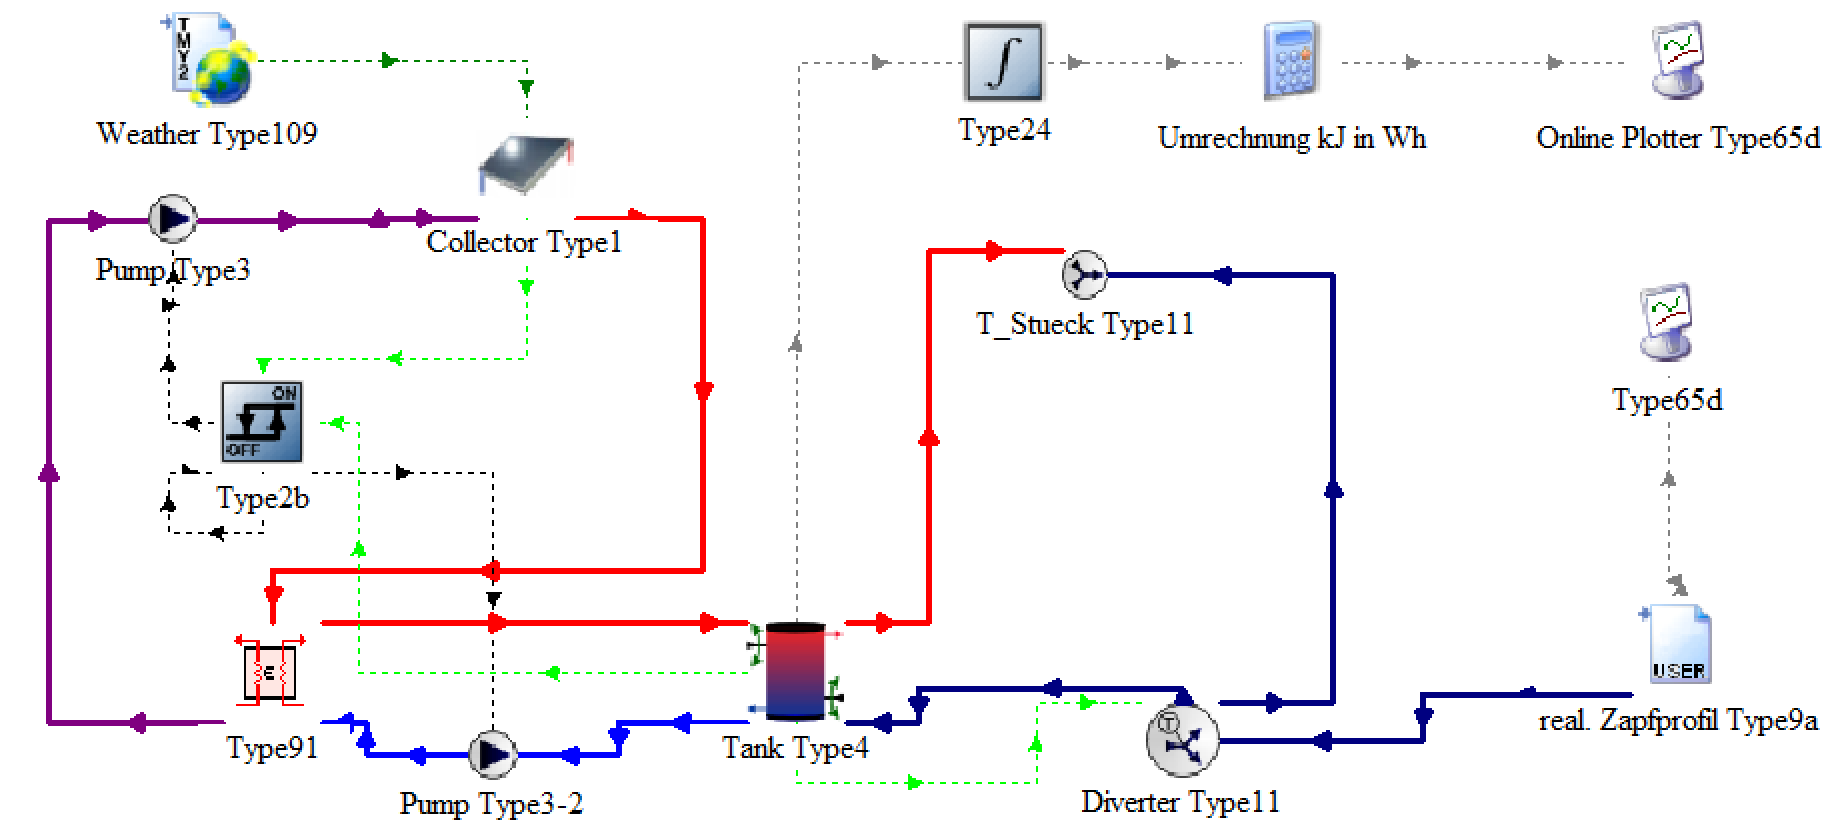
\includegraphics[width=0.8\textwidth]{../DATA/std_deck.png}
	\caption[Grundsystem]{Grundsystem des Decks}
	\label{fig:std_deck}
\end{figure}

Das System basiert auf einem Speicher mit integrierter Nachheizung und externem Wärmeübertrager, an welchen ein Kollektor mit Wetterdaten aus Stuttgart angeschlossen ist. Die Pumpen des Primär- und Sekundärkreislaufes des Wärmeübertragers werden per Temperaturdifferenzregelung angesteuert. Die Kollektortemperatur und die untere Speichertemperatur dienen dem Regler als Vergleichsgrößen. Die Regelung erfolgt als Ein- und Ausschaltsignal. Die Massenströme sind in den Pumpen selbst festgelegt. Ein Verteiler mit Zapfprofil versorgt den Speicher sowie einen Mischer mit Kaltwasser. Der Solare Wärmeeintrag in den Speicher und die Nachheizenergie werden über das Jahr integriert und graphisch ausgegeben.

\subsection{Systemanpassung: Rohrverluste und Kapazitätsströme}
Zur Erweiterung des Systems wird  zwischen dem Kollektor und dem Wärmeübertrager jeweils eine Rohrleitung in Vor- und Rücklauf installiert. Für Die Rohrlänge wurden \SI{9}{\meter} und für den Rohrdurchmesser \SI{2,5}{\centi\meter} angenommen, was zwei bis drei Etagenhöhen zuzüglich horizontaler Abschnitte und Verteilung auf dem Dach entspricht. Die Dicke der Dämmschicht wurde mit \SI{5}{\centi\meter} vorgegeben. Zur Bestimmung des Verlustkoeffizienten werden die Innenmantelfläche des Rohres sowie der UA-Wert benötigt. Der Wärmeleitkoeffizient des Kupferrohres wurde mit \SI{380}{\watt\per\meter\per\kelvin} angenommen.

\begin{equation}
	\label{eq:Arohr}
	A_{Rohr} = 2*\pi*r*h = 2*\pi*\SI{0,0125}{\meter}*\SI{9}{\meter}=\SI{0,70}{\square\meter}
\end{equation}

\begin{multline}
	\label{eq:UA}
UA = (\frac{1}{2*\pi*l}*(\frac{1}{\alpha_i*r_i}+\sum\frac{ln(\frac{r_{j+1}}{r_j})}{\lambda_j}+\frac{1}{\alpha_a*r_a}))^{-1} = (\frac{1}{2*\pi*\SI{9}{\meter}}\\*(\frac{1}{\SI{1000}{\watt\per\square\meter\per\kelvin}*\SI{0,0125}{\meter}}+\frac{ln(\frac{\SI{16}{\milli\meter}}{\SI{12,5}{\milli\meter}})}{\SI{380}{\watt\per\meter\per\kelvin}}+\frac{ln(\frac{\SI{66}{\milli\meter}}{\SI{16}{\milli\meter}})}{\SI{0,04}{\watt\per\meter\per\kelvin}}\\+\frac{1}{\SI{10}{\watt\per\meter\per\kelvin}*\SI{0,0666}{\meter}}))^{-1}=\SI{1,528}{\watt\per\kelvin}
\end{multline}


\begin{equation}
	\label{eq:U}
	U=\frac{UA}{A_{Rohr}}=\frac{\SI{1,528}{\watt\per\kelvin}}{\SI{0,70}{\square\meter}}=\SI{2,158}{\watt\per\square\meter\per\kelvin}
\end{equation}


Zur Anpassung der Kapazitätsströme wird der Massenstrom der sekundärseitigen Pumpe anhand des Quotienten der Wärmekapazitäten beider Fluide angepasst. Beide Pumpen werden weiterhin mit dem gleichen Regelsignal angesteuert:

\begin{equation}
	\label{eq:dotm}
	\dot m_{2}=\dot m_{1}*\frac{c_{p,1}}{c_{p,2}}
\end{equation}
Zusätzlich ist der benötigte Massenstrom von der Kollektorfläche abhängig. Um den Wärmetransport aus dem Kollektor auch bei größeren Flächen zu gewährleisten, wurde folgende Regelfunktion eingebaut:

\begin{equation}
	\label{eq:dotm2}
	\dot m_{1}=A_{kol}*\SI{20}{\kilogram\per\hour}
\end{equation}


\subsection{Systemauslegung}
Anhand der Wetterdaten von Stuttgart soll eine solare Deckung von \SI{60}{\percent} für das vorliegende Zapfprofil erzielt werden. Zunächst wurde eine Simulation ohne Kollektorfläche durchgeführt, um den Wärmebedarf des Systems zu ermitteln. Da die elektrische Nachheizung direkt im Kessel im Gegensatz zur Solaranlage kaum verlustbehaftet ist, eignet sich diese Methode zur Bedarfsbestimmung, ohne genauere Informationen über das Zapfprofil zu kennen. Mit steigendem $q_{sol}$ würde der Wärmebedarf entsprechend steigen. Der ermittelte Bedarf beträgt jährlich 2757\,kWh. Der solare Jahresertrag $q_{sol}$ wurde mit 350\,kWh pro m\textsuperscript{2} Kollektorfläche geschätzt. Daraus ergibt sich eine Kollektorfläche von

\begin{equation}
	\label{eq:}
	A_{kol}=\frac{Q_{Bedarf}*f_{sol}}{q_{sol}}=\frac{\SI{2757}{\kilo\watt\hour\per\square}*0,6}{\SI{350}{\kilo\watt\hour\per\square\meter}}=\SI{4,73}{\square\meter}
\end{equation}

Bei \SI{50}{\liter\per\square\meter} Speichervolumen entspricht dies einem 200..250\,l Speicher. Für die folgenden Simulationen wurden beide Größen auf \SI{5}{\square\meter} respektive \SI{300}{\liter} aufgerundet und eine Solare Deckung von

\begin{equation}
	\label{eq:fsolin}
	f_{sol,in} = \frac{Q_{sol}}{Q_{sol}+Q_{aux}} =\SI{67,7}{\percent}
\end{equation}
beziehungsweise
\begin{equation}
	\label{eqfsolout:}
	f_{sol,out} = \frac{Q_{sol}-Q_{verl,Sp}}{Q_{TWW+RH}+Q_{Zirk}}=\SI{61,7}{\percent}
\end{equation}
unter Berücksichtigung der Verluste erzielt.

\section{Parametervariation}
\subsection{Kaltwasser- und Umgebungstemperatur des Speichers}
Im Rahmen der Parametervariation wurden die Kaltwassertemperatur und die Umgebungstemperatur des Speicherraums in 5-Grad-Schritten von 5..30\si{\celsius} variiert. Insgesamt wurden somit 36 Simulationen durchgeführt. Abbildung \ref{fig:par1} zeigt die erzielte solare Deckung inklusive Verlusten.
\begin{figure}[H]
	\centering
	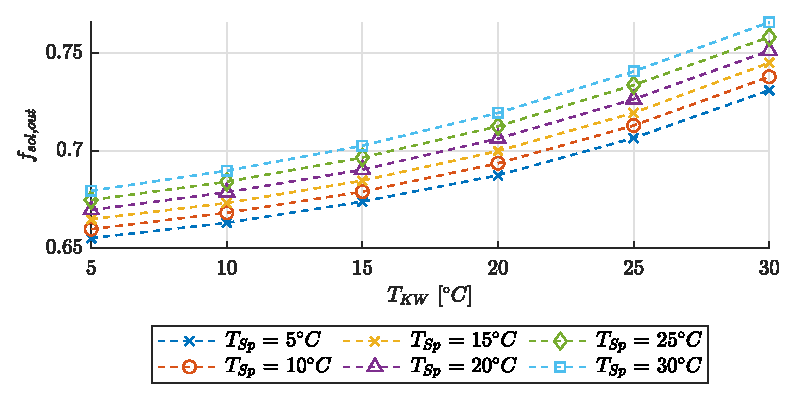
\includegraphics[width=0.8\textwidth]{../DATA/Aufgabe2.2.eps}
	\caption[Parametervariation Kaltwasser und Speicher]{Parametervariation Kaltwasser und Speicher}
	\label{fig:par1}
\end{figure}

Mit zunehmender Raumtemperatur und Kaltwassertemperatur steigt die solare Deckung an. Die Zulauftemperatur hat hierbei den größeren Einfluss von fast 10\,\%, da sie in direkt proportional in den Wärmebedarf einfließt. Die Speicherverluste spielen nur eine untergeordnete Rolle, da der Speicher gegen seine Umgebung isoliert ist. Innerhalb der Parametergrenzen unterscheidet sich die solare Deckung um etwa 3\,\%. Praktisch sind beide Einflussgrößen kaum beeinflussbar. Sowohl die Umgebungstemperatur als auch die Kaltwassertemperatur sind standortabhängig.

\subsection{Rohrlänge und Dämmung}
Die Parameter Rohrlänge, Dämmschichtdicke und Wärmeleitfähigkeit wurden jeweils einzeln variiert. Als Grundlage wurden stets die bereits zuvor verwendeten Parameter genutzt und von dort ausgehend immer ein Parameter nach oben und unten variiert.  Zunächst wurde der Einfluss der Rohrlänge betrachtet. Da das System aus Vor- und Rücklauf besteht, muss die X-Achse gedoppelt werden. Mit steigenden Rohrlängen sinkt der solare Ertrag (innerhalb der gewählten Parametergrenzen) näherungsweise linear. Längere Leitungen wurden aufgrund der geringen Anlagengröße nicht betrachtet. Allerdings ist zu berücksichtigen, dass die Rohre in der Standardkonfiguration bereits über eine gute Dämmung verfügen. Eine schlechtere Dämmung hätte einen größeren Einfluss der Rohrlänge zur Folge.

Bei der Variation der Dämmstärke wurde der aktuelle Baustandard berücksichtigt. Die Parametergrenzen entsprechen dem halben bis vierfachen Rohrinnendurchmesser. Eine Dämmstärke des einfachen Durchmessers ist Voraussetzung für energieeffizientes Bauen, für Passivhäuser wird eine Dämmstärke bis zum doppelten Rohrdurchmesser empfohlen. Bereits ab diesem Wert sinkt der Einfluss der Dämmung und die zusätzlichen Gewinne werden geringer. Die Wirkung der Dämmung ist jedoch auch von der Wärmeleitfähigkeit abhängig. Bei schlechterer Isolierwirkung würde der Verlauf der Dämmstärke weniger abflachen. Die genannten Empfehlungen zur Dämmstärke sind für einen Wärmeleitungskoeffizienten von \SI{0,035}{\watt\per\meter\per\kelvin} gültig.

Bei der Variation der Wärmeleitfähigkeit wurden Werte von gängigen Dämmstoffen herangezogen. Wie bei der Rohrlänge ist auch hier ein näherungsweise linearer Abfall zu beobachten.

Für eine möglichst hohe solare Deckung ist die richtige Auslegung aller Einflussgrößen sehr wichtig, da jeder Parameter für sich innerhalb realistisch gewählter Größenordnungen bereits Verluste bis zu \SI{10}{\percent} hervorrufen kann. Das größte Potential liegt theoretisch betrachtet in der Wahl des Dämmmaterials, da die solare Deckung sich weiter Steigern lässt. Lediglich die Verfügbarkeit und Kosten schränken diesen Faktor ein. Die Rohrlänge wird von den baulichen Gegebenheiten festgelegt, die Dämmstärke unterliegt einem Sättigungseffekt.

\begin{figure}[H]
	\centering
	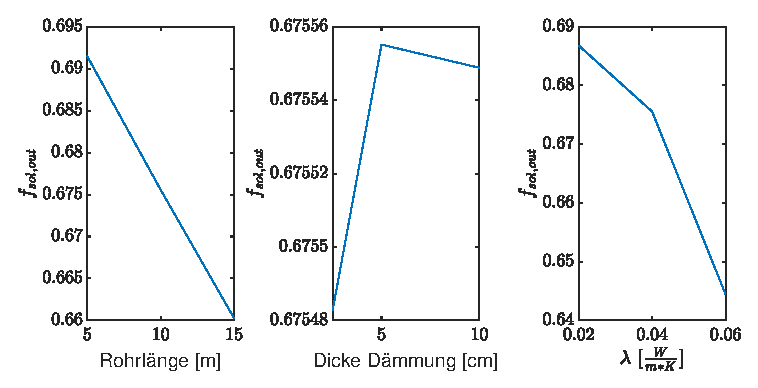
\includegraphics[width=0.8\textwidth]{../DATA/Aufgabe2.3.eps}
	\caption[Parametervariation Dämmung]{Parametervariation Dämmung}
	\label{fig:par2}
\end{figure}


\section{Optimierung der Kollektorparameter}

Abbildung \ref{fig:comp} zeigt folgendes bli bla blub.

\begin{figure}[H]
	\centering
	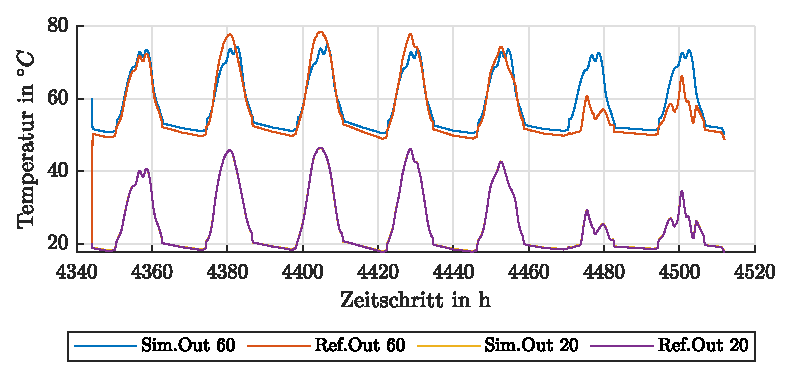
\includegraphics[width=0.8\textwidth]{../DATA/Aufgabe3vergleich.eps}
	\caption[Vergleich Optimierung-Referenz]{Vergleich der Simulation optimierter Parameter mit der Referenzmessung.}
	\label{fig:comp}
\end{figure}

